\subsection{Núcleo Triangulum: Comunicação de Profundidade}

\begin{figure}[!htbp]
\centering
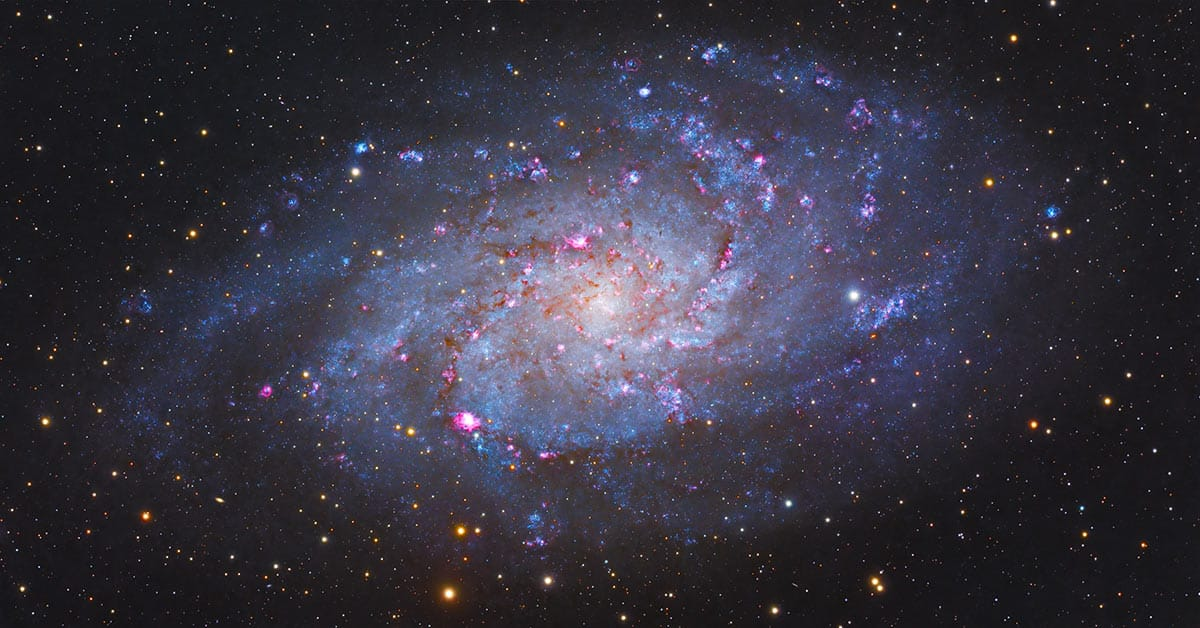
\includegraphics[width=1\linewidth]{files/triangulum-6481214de20cda52c86e4ba5076d2476.jpg}
\end{figure}

\subsubsection{Visão Geral}

O \textbf{Núcleo Triangulum} é responsável pela comunicação de profundidade e autoridade científica do Projeto Hermathena. Seu nome evoca a galáxia do Triângulo, símbolo de exploração profunda do cosmos, representando nosso compromisso com conteúdo aprofundado, documentários e produções que exigem tempo e expertise.

\subsubsection{Missão}

Produzir conteúdo audiovisual e jornalístico de alta qualidade que aprofunde o conhecimento científico sobre o BINGO e a cosmologia, estabelecendo o projeto como referência em divulgação científica no Brasil.

\subsubsection{Objetivos Específicos}

\paragraph{1. Podcasts e Áudio}

\subparagraph{1.1 ``RadioBingo'' - Podcast Principal}

\begin{itemize}
\item \textbf{Formato:} Notícias - Entrevista/Conteúdo Aprofundado
\item \textbf{Duração:} 20 minutos
\item \textbf{Frequência:} Quinzenal (2 episódios/mês)
\item \textbf{Plataformas:} Spotify, Apple Podcasts, Deezer, YouTube
\item \textbf{Estrutura:}

\begin{itemize}
\item Introdução (5 min) - Notícias da astronomia
\item Entrevista (13 min) - Tema aprofundado
\item Encerramento (2 min) - Próximos episódios e CTA
\end{itemize}
\end{itemize}

\subparagraph{1.2 ``BINGO Minuto'' - Micro-podcast}

\begin{itemize}
\item \textbf{Formato:} Notícias rápidas e curiosidades
\item \textbf{Duração:} 5-8 minutos
\item \textbf{Frequência:} Quinzenal
\item \textbf{Conteúdo:} Atualizações do projeto, explicações curtas, Notícias
\end{itemize}

\subparagraph{1.3 ``Mesa do Sertão'' - Conversas informais}

\begin{itemize}
\item \textbf{Formato:} Debates em mesa-redonda
\item \textbf{Duração:} 45 minutos
\item \textbf{Frequência:} Mensal
\item \textbf{Tema:} Ciência, cultura e desenvolvimento regional
\end{itemize}

\paragraph{2. Canal no YouTube}

\subparagraph{2.1 Séries de Conteúdo}

\textbf{Série ``Construindo o BINGO'' (Documental)}

\begin{itemize}
\item 12 episódios de 10-15 minutos
\item Acompanhamento da construção do telescópio
\item Entrevistas com engenheiros e técnicos
\item Lançamento: 1 episódio por mês
\end{itemize}

\textbf{Série ``Cosmologia para Todos'' (Educativa)}

\begin{itemize}
\item Vídeos de 8-12 minutos
\item Conceitos fundamentais explicados visualmente
\item Animações e infográficos
\item Frequência: 1 x por mês
\end{itemize}

\textbf{Série ``Pergunte ao Cientista'' (Q\&A)}

\begin{itemize}
\item Respostas em vídeo a perguntas do público
\item Duração: 5-10 minutos
\item Frequência: Semanal
\item Fonte: Perguntas das redes sociais
\end{itemize}

\subparagraph{2.2 Lives e Transmissões}

\bigskip\noindent
\begin{tabular}{p{\dimexpr 0.250\linewidth-2\tabcolsep}p{\dimexpr 0.250\linewidth-2\tabcolsep}p{\dimexpr 0.250\linewidth-2\tabcolsep}p{\dimexpr 0.250\linewidth-2\tabcolsep}}
\toprule
Evento & Frequência & Duração & Conteúdo \\
\hline
Live mensal & trimestral & 1 hora & Tema livre com Q\&A \\
Webinários técnicos & 2x/ano & 2 horas & Seminários científicos \\
Cobertura de eventos & Eventuais & Variável & Feiras, workshops, inaugurações \\
\bottomrule
\end{tabular}

\bigskip

\paragraph{3. Documentários}

\subparagraph{3.1 Documentário Principal: ``BINGO: Olhos no Sertão''}

\begin{itemize}
\item \textbf{Duração:} 45-60 minutos
\item \textbf{Formato:} Documentário científico
\item \textbf{Lançamento:} Final do primeiro ano
\item \textbf{Sinopse:} A história do primeiro radiotelescópio de grande porte do Brasil, desde sua concepção até as primeiras observações
\item \textbf{Distribuição:} YouTube, streaming educacional, TVs públicas
\end{itemize}

\subparagraph{3.2 Documentários Curtos (15 min)}

\bigskip\noindent
\begin{tabular}{p{\dimexpr 0.333\linewidth-2\tabcolsep}p{\dimexpr 0.333\linewidth-2\tabcolsep}p{\dimexpr 0.333\linewidth-2\tabcolsep}}
\toprule
Título & Tema & Prazo \\
\hline
``A Escolha do Sertão'' & Por que Aguiar foi escolhido & Mês 6 \\
``Engenheiros do Impossível'' & Desafios técnicos da construção & Mês 8 \\
``Olhando o Invisível'' & Como a radioastronomia funciona & Mês 10 \\
``O Futuro Começa Aqui'' & Impacto do BINGO para o Brasil & Mês 12 \\
\bottomrule
\end{tabular}

\bigskip

\paragraph{4. Webinários e Seminários}

\subparagraph{4.1 Ciclo de Palestras BINGO}

\begin{itemize}
\item \textbf{Frequência:} Mensal
\item \textbf{Formato:} Palestra online com Q\&A
\item \textbf{Público:} Estudantes e pesquisadores
\item \textbf{Palestrantes:} Membros da colaboração BINGO
\item \textbf{Temas sugeridos:}

\begin{itemize}
\item ``Introdução à Cosmologia''
\item ``Energia Escura: O Mistério do Universo''
\item ``Radioastronomia: Uma Nova Janela''
\item ``Os BAO e a Escala do Universo''
\item ``Tecnologia do BINGO''
\end{itemize}
\end{itemize}

\subparagraph{4.2 Seminário Anual de Divulgação Científica}

\begin{itemize}
\item \textbf{Frequência:} Anual
\item \textbf{Duração:} 2 dias
\item \textbf{Formato:} Híbrido (presencial e online)
\item \textbf{Público:} Educadores, comunicadores, estudantes
\item \textbf{Atividades:} Palestras, workshops, mostra de trabalhos
\end{itemize}

\paragraph{5. Jornalismo Científico}

\subparagraph{5.1 Artigos Especiais}

\textbf{Blog Hermathena}

\begin{itemize}
\item Artigos longos (1.500-3.000 palavras)
\item Profundidade científica acessível
\item Frequência: 2x por mês
\item Temas:

\begin{itemize}
\item ``A História das BAO''
\item ``O Telescópio que Veio da China''
\item ``Cientistas Paraibanos no BINGO''
\item ``O Legado do Radiotelescópio''
\end{itemize}
\end{itemize}

\subparagraph{5.2 Reportagens}

\begin{itemize}
\item Cobertura jornalística de eventos
\item Entrevistas exclusivas com cientistas internacionais
\item Reportagens especiais para veículos de comunicação parceiros
\end{itemize}

\subsubsection{Estrutura de Produção}

\paragraph{Estúdio Mínimo Necessário}

\bigskip\noindent
\begin{tabular}{p{\dimexpr 0.333\linewidth-2\tabcolsep}p{\dimexpr 0.333\linewidth-2\tabcolsep}p{\dimexpr 0.333\linewidth-2\tabcolsep}}
\toprule
Equipamento & Especificação & Finalidade \\
\hline
\textbf{Câmera principal} & Sony ZV-E10 ou similar & Gravação de vídeo \\
\textbf{Lentes} & 16-50mm f/3.5-5.6 + 50mm f/1.8 & Versatilidade e baixa luz \\
\textbf{Microfone principal} & Tascam TM-70 ou similar & Áudio de qualidade \\
\textbf{Mixer áudio} & Tascam Mixcast 4 & Podcasts e lives \\
\textbf{Iluminação} & Kit softbox LED 3 pontos & Iluminação controlada \\
\textbf{Tripé} & Tripé profissional + gimbal & Estabilidade \\
\textbf{Fones} & Tascam TH-05 ou similar & Monitoramento \\
\textbf{Gravador portátil} & Zoom H1n & Entrevistas em campo \\
\bottomrule
\end{tabular}

\bigskip

\paragraph{Software de Produção}

\bigskip\noindent
\begin{tabular}{p{\dimexpr 0.333\linewidth-2\tabcolsep}p{\dimexpr 0.333\linewidth-2\tabcolsep}p{\dimexpr 0.333\linewidth-2\tabcolsep}}
\toprule
Categoria & Ferramenta & Uso \\
\hline
Edição de vídeo & Adobe Premiere Pro & Montagem final \\
Edição de áudio & Adobe Audition & Pós-produção sonora \\
Motion graphics & After Effects & Animações e vinhetas \\
Color grading & DaVinci Resolve & Correção de cor \\
Design gráfico & Photoshop/Illustrator & Thumbnails e artes \\
Gestão de projetos & Notion/Trello & Organização \\
\bottomrule
\end{tabular}

\bigskip

\paragraph{Fluxo de Produção de Documentário}

\begin{verbatim}
┌─────────────────┐    ┌─────────────────┐    ┌─────────────────┐
│ 1. PRÉ -PRODUÇÃO │ -> │ 2. PRODUÇÃO     │ -> │ 3. PÓS -PRODUÇÃO │
│                 │    │                 │    │                 │
│ \cdot Pesquisa      │    │ \cdot Filmagens     │    │ \cdot Edição        │
│ \cdot Roteiro       │    │ \cdot Entrevistas   │    │ \cdot Áudio         │
│ \cdot Planejamento  │    │ \cdot B -roll        │    │ \cdot Finalização   │
│ \cdot Permissões    │    │ \cdot Áudio         │    │ \cdot Legendas      │
└─────────────────┘    └─────────────────┘    └─────────────────┘
        │                                              │
        v                                              v
┌─────────────────┐                         ┌─────────────────┐
│ 4. REVISÃO      │ < -                      │ 5. DISTRIBUIÇÃO │
│                 │                         │                 │
| \cdot Validação     │                         │ \cdot YouTube       │
│   científica    │                         │ \cdot Podcasts      │
| \cdot Ajustes       │                         │ \cdot Imprensa      │
└─────────────────┘                         └─────────────────┘
\end{verbatim}

\subsubsection{Cronograma de Produção (Ano 1)}

\paragraph{Trimestre 1: Setup e Primeiras Produções}

\bigskip\noindent
\begin{tabular}{p{\dimexpr 0.333\linewidth-2\tabcolsep}p{\dimexpr 0.333\linewidth-2\tabcolsep}p{\dimexpr 0.333\linewidth-2\tabcolsep}}
\toprule
Semana & Atividade & Entregável \\
\hline
1-2 & Aquisição e setup de equipamentos & Estúdio funcional \\
3-4 & Testes e gravações piloto & Episódios pilotos \\
5-6 & Lançamento podcast ``Cosmos em Foco'' & 2 episódios no ar \\
7-8 & Lançamento canal YouTube & 4 vídeos publicados \\
9-10 & Primeiras lives & 2 transmissões \\
11-12 & Análise e ajustes & Relatório de aprendizados \\
\bottomrule
\end{tabular}

\bigskip

\paragraph{Trimestre 2-4: Consolidação}

\bigskip\noindent
\begin{tabular}{p{\dimexpr 0.333\linewidth-2\tabcolsep}p{\dimexpr 0.333\linewidth-2\tabcolsep}p{\dimexpr 0.333\linewidth-2\tabcolsep}}
\toprule
Trimestre & Foco & Meta \\
\hline
\textbf{T2} & Consolidação de formatos & 6 episódios podcast, 12 vídeos \\
\textbf{T3} & Expansão de conteúdo & Webinários, parcerias \\
\textbf{T4} & Documentário principal & Finalização e lançamento \\
\bottomrule
\end{tabular}

\bigskip

\subsubsection{Métricas de Sucesso}

\paragraph{Indicadores Quantitativos}

\bigskip\noindent
\begin{tabular}{p{\dimexpr 0.333\linewidth-2\tabcolsep}p{\dimexpr 0.333\linewidth-2\tabcolsep}p{\dimexpr 0.333\linewidth-2\tabcolsep}}
\toprule
Plataforma & Indicador & Meta Ano 1 \\
\hline
Spotify & Downloads mensais & 500 \\
YouTube & Inscritos & 2.000 \\
YouTube & Visualizações/mês & 5.000 \\
YouTube & Horas de exibição & 500/mês \\
Lives & Espectadores simultâneos & 100 \\
Blog & Visitas/mês & 1.000 \\
\bottomrule
\end{tabular}

\bigskip

\paragraph{Indicadores Qualitativos}

\begin{itemize}
\item \textbf{Retenção de audiência:} \textgreater 50\% do vídeo assistido
\item \textbf{Comentários qualificados:} Perguntas e debates significativos
\item \textbf{Citações em mídia:} Referências ao conteúdo produzido
\item \textbf{Engajamento educacional:} Uso em sala de aula
\end{itemize}

\subsubsection{Parcerias de Conteúdo}

\paragraph{Institucionais}

\bigskip\noindent
\begin{tabular}{p{\dimexpr 0.333\linewidth-2\tabcolsep}p{\dimexpr 0.333\linewidth-2\tabcolsep}p{\dimexpr 0.333\linewidth-2\tabcolsep}}
\toprule
Parceiro & Tipo de Parceria & Contribuição \\
\hline
USP/INPE & Entrevistados & Cientistas para podcasts \\
UEPB/UFPB & Co-produção & Conteúdo regional \\
TVs Universitárias & Distribuição & Exibição de documentários \\
Rádios locais & Áudio & Transmissão de podcasts \\
\bottomrule
\end{tabular}

\bigskip

\paragraph{Comerciais}

\bigskip\noindent
\begin{tabular}{p{\dimexpr 0.333\linewidth-2\tabcolsep}p{\dimexpr 0.333\linewidth-2\tabcolsep}p{\dimexpr 0.333\linewidth-2\tabcolsep}}
\toprule
Parceiro & Tipo & Benefício \\
\hline
Spotify & Plataforma & Distribuição \\
YouTube & Plataforma & Monetização futura \\
Padlet/Escolas & Distribuição & Alcance educacional \\
\bottomrule
\end{tabular}

\bigskip

\subsubsection{Estrutura da Equipe}

\bigskip\noindent
\begin{tabular}{p{\dimexpr 0.333\linewidth-2\tabcolsep}p{\dimexpr 0.333\linewidth-2\tabcolsep}p{\dimexpr 0.333\linewidth-2\tabcolsep}}
\toprule
Função & Quantidade & Perfil \\
\hline
\textbf{Professor Orientador} & 1 & Docente Comunicação/Cinema \\
\textbf{Professor Colaborador} & 1 & Docente área complementar \\
\textbf{Bolsista PROBEX} & 1 & Graduação Comunicação/Cinema \\
\textbf{Voluntários} & 5 & Graduação em áreas afins \\
\bottomrule
\end{tabular}

\bigskip

\textbf{Total por núcleo:} 8 pessoas

\textbf{Expansão:} Pode replicar em instituições parceiras (até 12 alunos + 4 docentes)

\subsubsection{Orçamento Estimado (Ano 1)}

\bigskip\noindent
\begin{tabular}{p{\dimexpr 0.500\linewidth-2\tabcolsep}p{\dimexpr 0.500\linewidth-2\tabcolsep}}
\toprule
Categoria & Valor (R\$) \\
\hline
Bolsa (1 bolsista $\times$ 6 meses $\times$ R\$ 400) & 2.400,00 \\
Equipamentos (câmera, áudio, iluminação) & 20.000,00 \\
Software e assinaturas & 3.000,00 \\
Produção de documentário & 8.000,00 \\
Deslocamentos para gravações & 5.000,00 \\
Infraestrutura de estúdio & 4.000,00 \\
\textbf{Total} & \textbf{48.400,00} \\
\bottomrule
\end{tabular}

\bigskip

\subsubsection{Referências e Benchmarking}

\paragraph{Canais de Referência}

\bigskip\noindent
\begin{tabular}{p{\dimexpr 0.333\linewidth-2\tabcolsep}p{\dimexpr 0.333\linewidth-2\tabcolsep}p{\dimexpr 0.333\linewidth-2\tabcolsep}}
\toprule
Canal & Plataforma & O que aprender \\
\hline
Canal do Pirulla & YouTube & Divulgação científica acessível \\
SciShow & YouTube & Produção ágil e consistente \\
RadioLab & Podcast & Narrativa sonora \\
Nerdologia & YouTube & Hibridização cultura pop + ciência \\
Space Today & YouTube & Cobertura de astronomia \\
Vox & YouTube & Produção visual de alta qualidade \\
\bottomrule
\end{tabular}

\bigskip


\bigskip
\centerline{\rule{13cm}{0.4pt}}
\bigskip

\textit{Documento sujeito a ajustes conforme evolução da produção.}